\chapter{RESULTS}

\section{Model Constraints and Curation}


To make sure the \emph{in-silico} growth rate predictions are in agreement with the physiological kinetic parameters obtained from the laboratory experiments, fine adjustment on the chosen metabolic model is a requirement. Since the growth-associated maintenance (GAM) and non-growth associated maintenance (NGAM) reactions in a model play a determinant role in the simulation results, fluxes through these reactions must be constrained to a fixed value. Flux of the NGAM reaction is constrained to 0.7 mmol gDWh\textsuperscript{-1} for aerobic model, and 0 mmol gDWh\textsuperscript{-1} for anaerobic model simulations as calculated in the previous studies \cite{nilsson2016metabolic}. Since the GAM depends on the biomass composition defined, results of a chemostat experiment \cite{van1998effect} are used as a guide to fit simulation predictions to. The model is simulated iteratively with a range of values for the GAM and the best fit is found at the level of 31.4 mmol gDWh\textsuperscript{-1} (Figure \ref{fig:gam_fitting}).

\begin{figure}[H]
  \begin{center}
  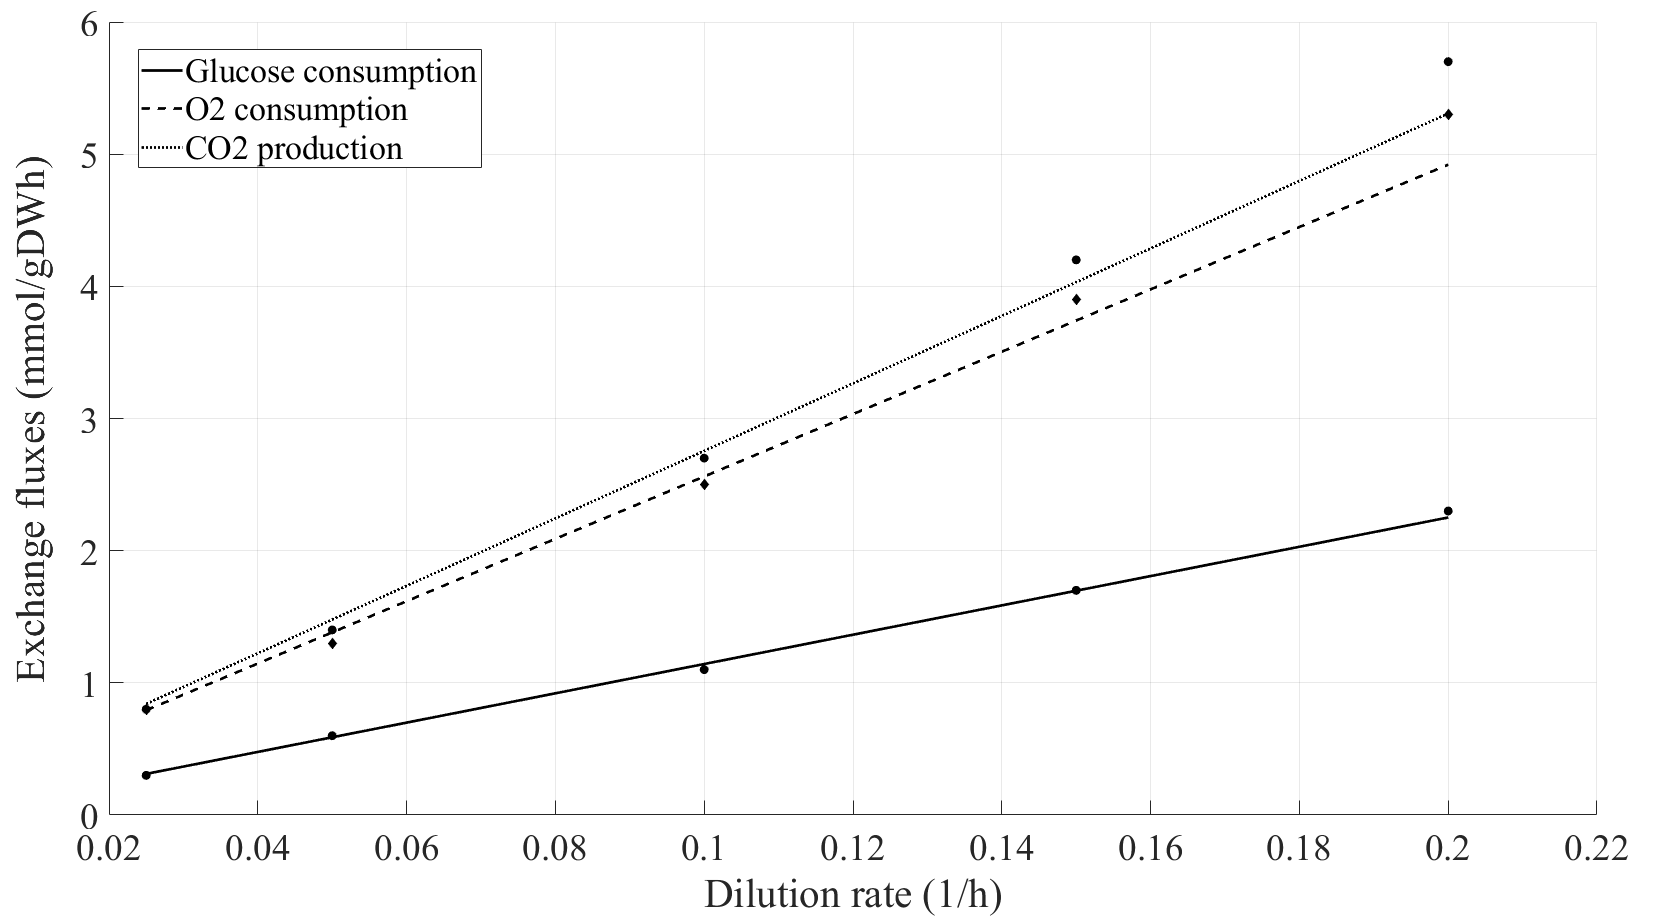
\includegraphics[width=1\columnwidth]{figures/gamfitting.png}
  \caption[Growth associated maintenance fitting]{Growth associated maintenance fitting results.}
  \end{center}
  \label{fig:gam_fitting}
\end{figure}

Average enzyme saturation value is set to 50\% where the lowest error rate is obtained as a fraction to biomass (Figure \ref{fig:sigma_fitting}). By constraining the total enzyme mass, the metabolic model became able to show overflow metabolism without any other constaint applied.

\begin{figure}[H]
  \begin{center}
  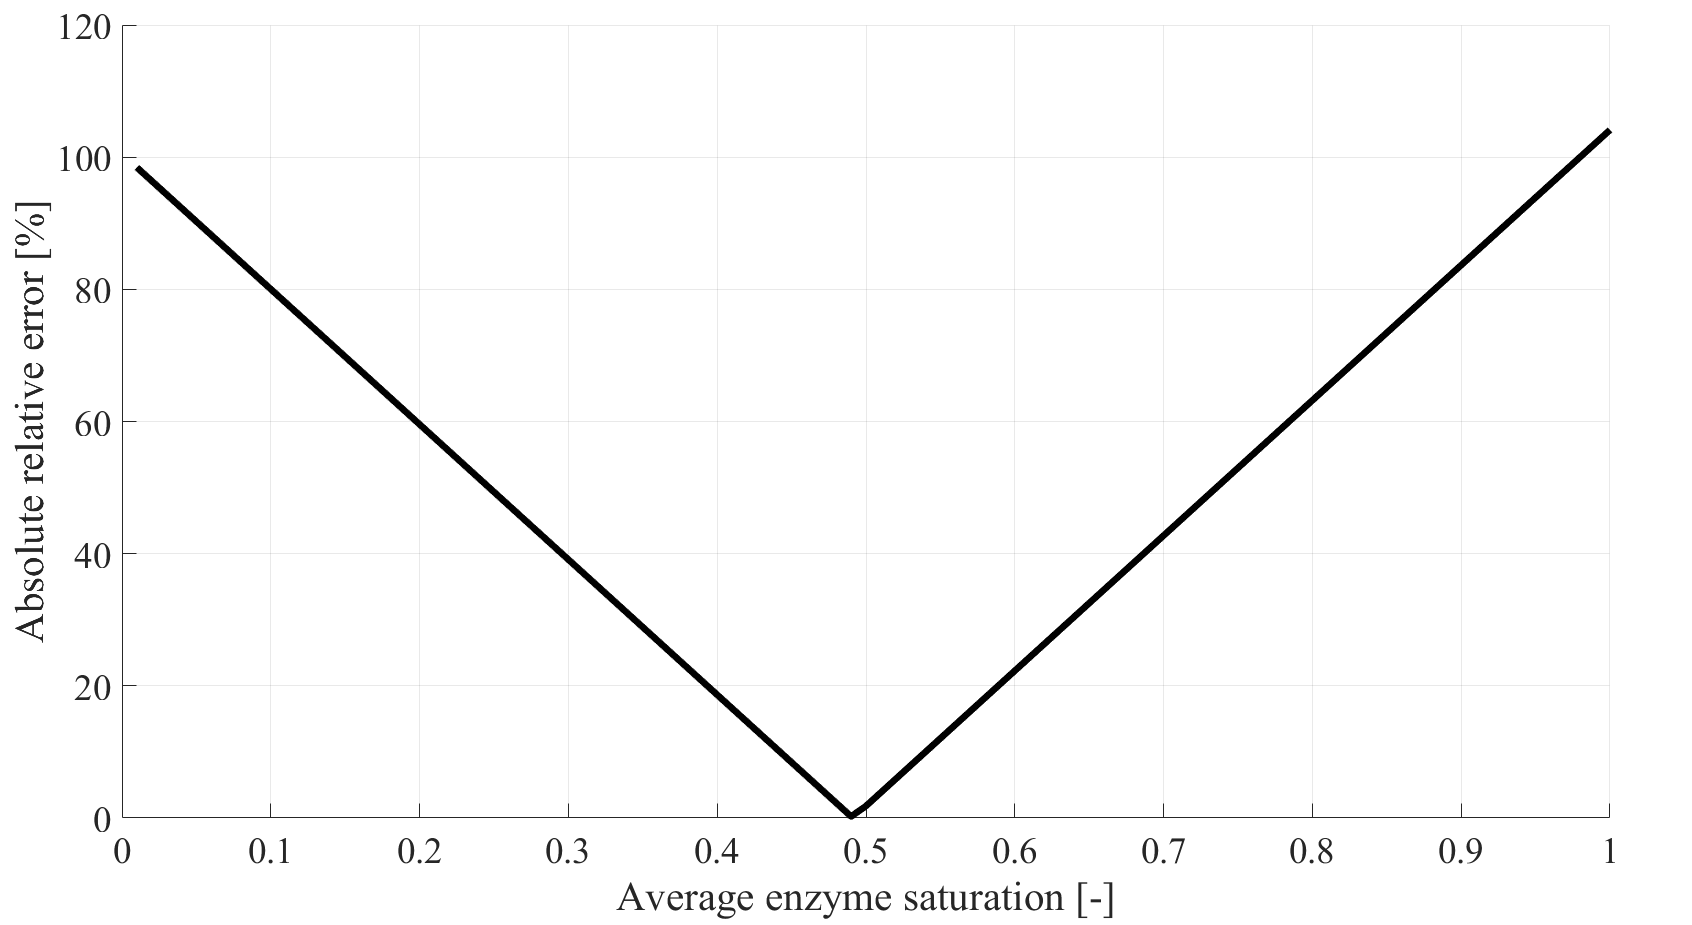
\includegraphics[width=1\columnwidth]{figures/sigmafitting.png}
  \caption[Average enzyme saturation factor fitting]{Average enzyme saturation factor fitting results.}
  \end{center}
  \label{fig:sigma_fitting}
\end{figure}

To prevent over-constraining the model with the enzyme kinetics, the most limiting proteins in the model are found based on their sensitivity on the objective function, i.e. growth. The $k_{cat}$ values for the the limiting enzymes are updated with the maximum available values from BRENDA\cite{jeske2019brenda} database by automated iterations until the simulation results for the growth rate agrees with the experimental growth rate. Modifications to the $k_{cat}$ values with their objective control coefficients can be found in the Table \ref{table:gecko_iterations}.

\begin{table}[H]
  \begin{center}
  \caption[Iterations on the network to find the top limiting proteins by their objective control coefficients (cc), i.e. sensitivities on the growth, with previous and updated $k_{cat}$ values and error improvements]{Iterations on the network to find the top limiting proteins by their objective control coefficients (cc), i.e. sensitivities on the growth, with previous and updated $k_{cat}$ values and error improvements. }
  \vskip0.5\baselineskip
  \begin{tabular}{ccp{5cm}cccc}
     \hline
    \textbf{\#} & \textbf{Protein} & \textbf{Reaction Name} & \textbf{prev $k_{cat}$} & \textbf{new $k_{cat}$} & \textbf{CC} & \textbf{Err\%}  \\
      \hline
      1 & P38604 & lanosterol synthase & 0.002 & 4.076 & 0.937 & -42.6 \\ \hline
      2 & P38972 & 5'-phosphoribosylformyl \newline glycinamidine synthetase & 0.05 & 5.07 & 0.244 & -28.7 \\   \hline
      3 & P00931 & tryptophan synthase \newline (indoleglycerol phosphate) & 0.022 & 775.75 & 0.129 & -19.4 \\   \hline
      4 & P48445 & acetyl-CoA carboxylase & 1.23 & 450000 & 0.065 & -14.2 \\   \hline
      5 & P05694 & methionine synthase & 0.33 & 3.5 & 0.050 & -10.3 \\   \hline
      6 & P39006 & PS decarboxylase \newline (1-16:1, 2-16:1) & 0.053 & 366.667 & 0.043 & -6.4 \\   \hline
  \end{tabular}
  \label{table:gecko_iterations}
  \end{center}
\end{table}


\vspace{-0.5cm}
\section{Differential Expression Analysis and Integration}

The obtained expression datasets were quantile-normalized. Three replicates for both reference and the evolved strains for each experiment (exception with the ethanol-b8 strain which has two replicates) is used for the differential analysis. The distribution across normalized gene expression levels across each experiment can be seen in the Figure \ref{fig:expr_boxplot}.

\begin{figure}[H]
\begin{center}
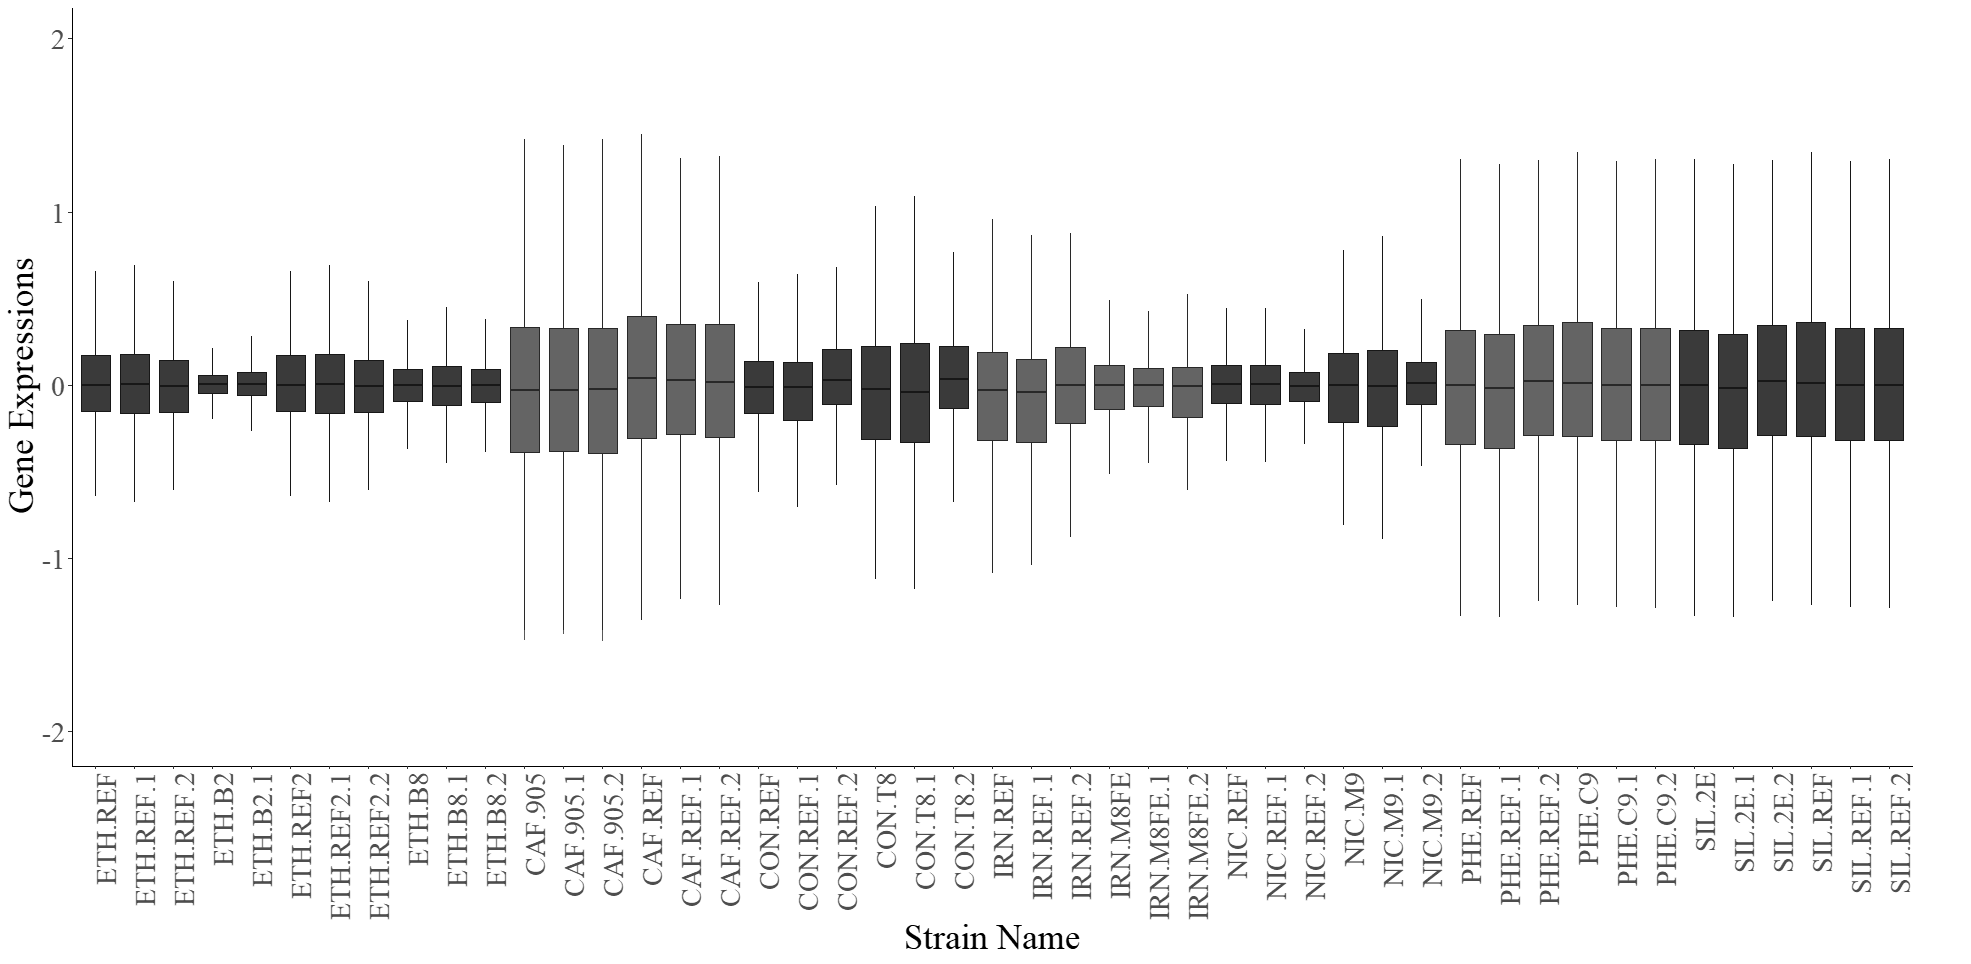
\includegraphics[width=1\columnwidth]{figures/expr_boxplots.png}
\caption[Boxplots of the normalized gene expression levels]{Boxplots of the normalized gene expression levels obtained from Gene Expression Omnibus.}
\end{center}
\label{fig:expr_boxplot}
\end{figure}

A statistical threshold (p $<$ 0.05) for the differential analysis of the normalized gene expression levels detected a total of 1606 genes in ethanol-b2, 2947 genes in ethanol-b8, 4743 genes in caffeine, 2267 genes in coniferylaldehyde, 3448 genes in iron, 152 genes in nickel, 4796 genes in phenylethanol, and 4796 genes in silver resistant strains differentially expressed. Commonly upregulated and downregulated genes frequencies across all strains can be found in the Figure \ref{fig:intersections_genes}.

\begin{figure}[H]
\begin{center}
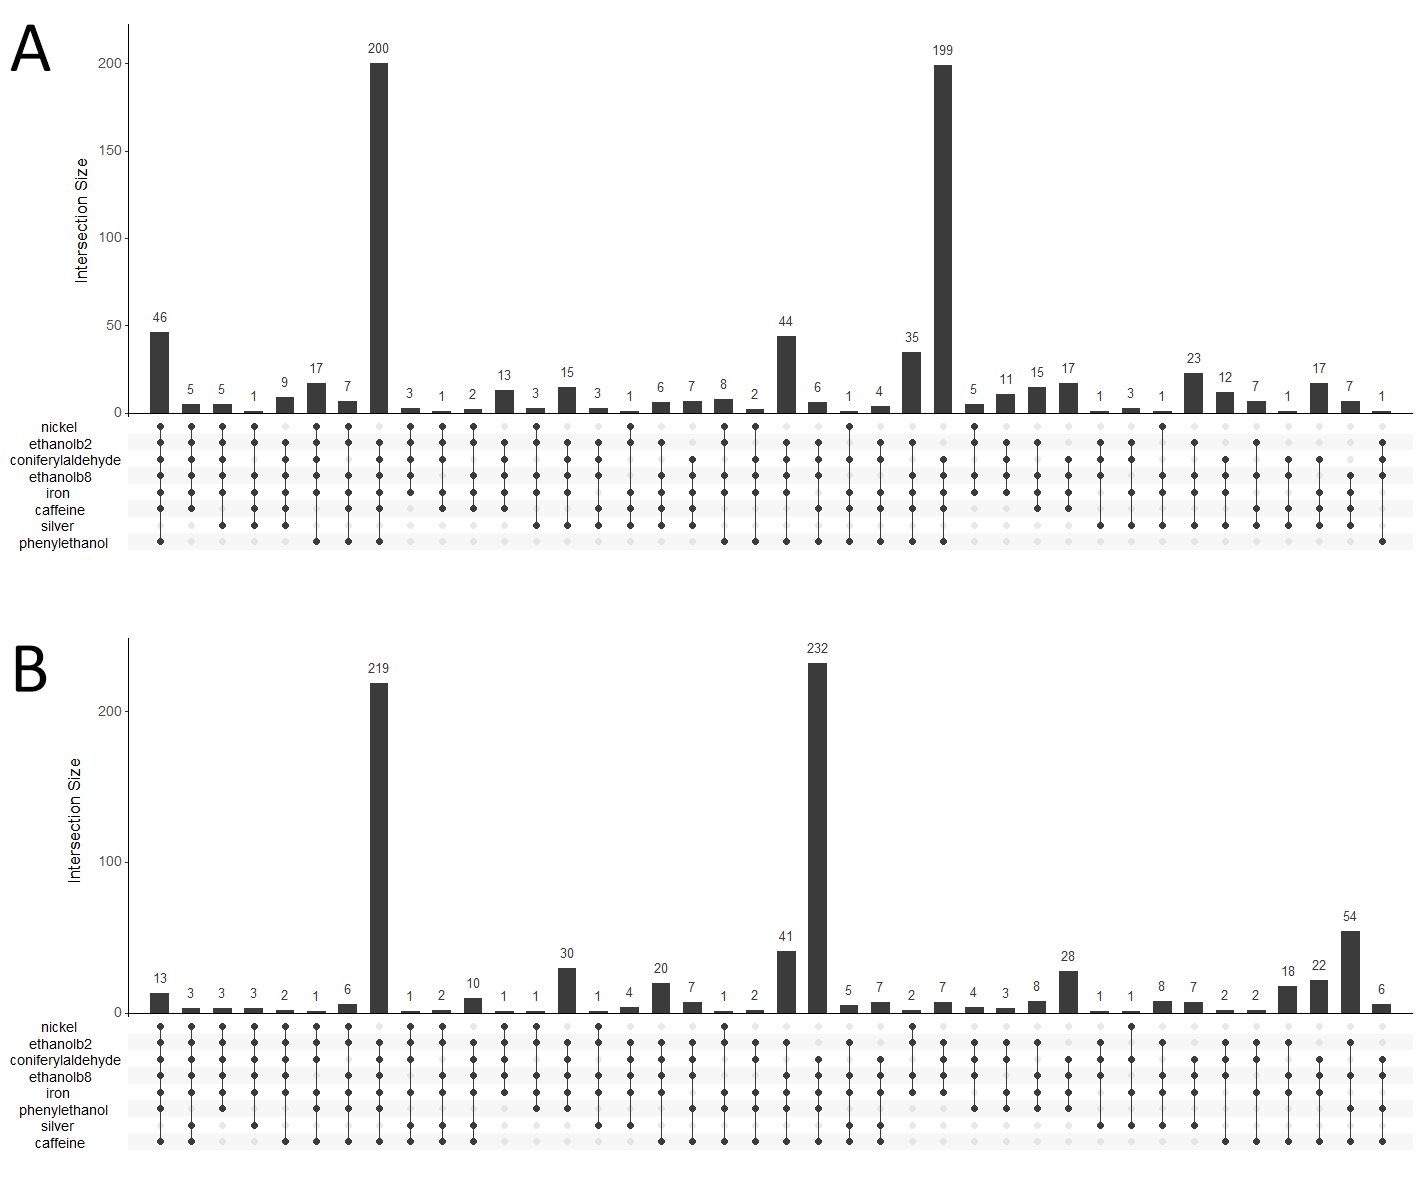
\includegraphics[width=1\columnwidth]{figures/intersections_by_degree.png}
\caption[Differential gene expression intersections across experiments]{Differential gene expression intersections across experiments. (A) Upregulated, (B) downregulated gene frequencies.}
\end{center}
\label{fig:intersections_genes}
\end{figure}

The log2(fold-change) values of differentially expressed genes and their frequencies are plotted for each experiment in Figure \ref{fig:expr_frequencies}. Although the high number of differentially expressed genes are collected, due to the limited reaction number in the genome-scale metabolic model, only a part of obtained fold-change expression values are integrated into model. Total of 277 genes in ethanol-b2, 464 genes in ethanol-b8, 783 genes in caffeine, 374 genes in coniferylaldehyde, 552 genes in iron, 28 genes in nickel, 759 genes in phenylethanol and 759 genes in silver resistant strains were integrated into the metabolic model to generate strain-specific models.

\begin{figure}[H]
\begin{center}
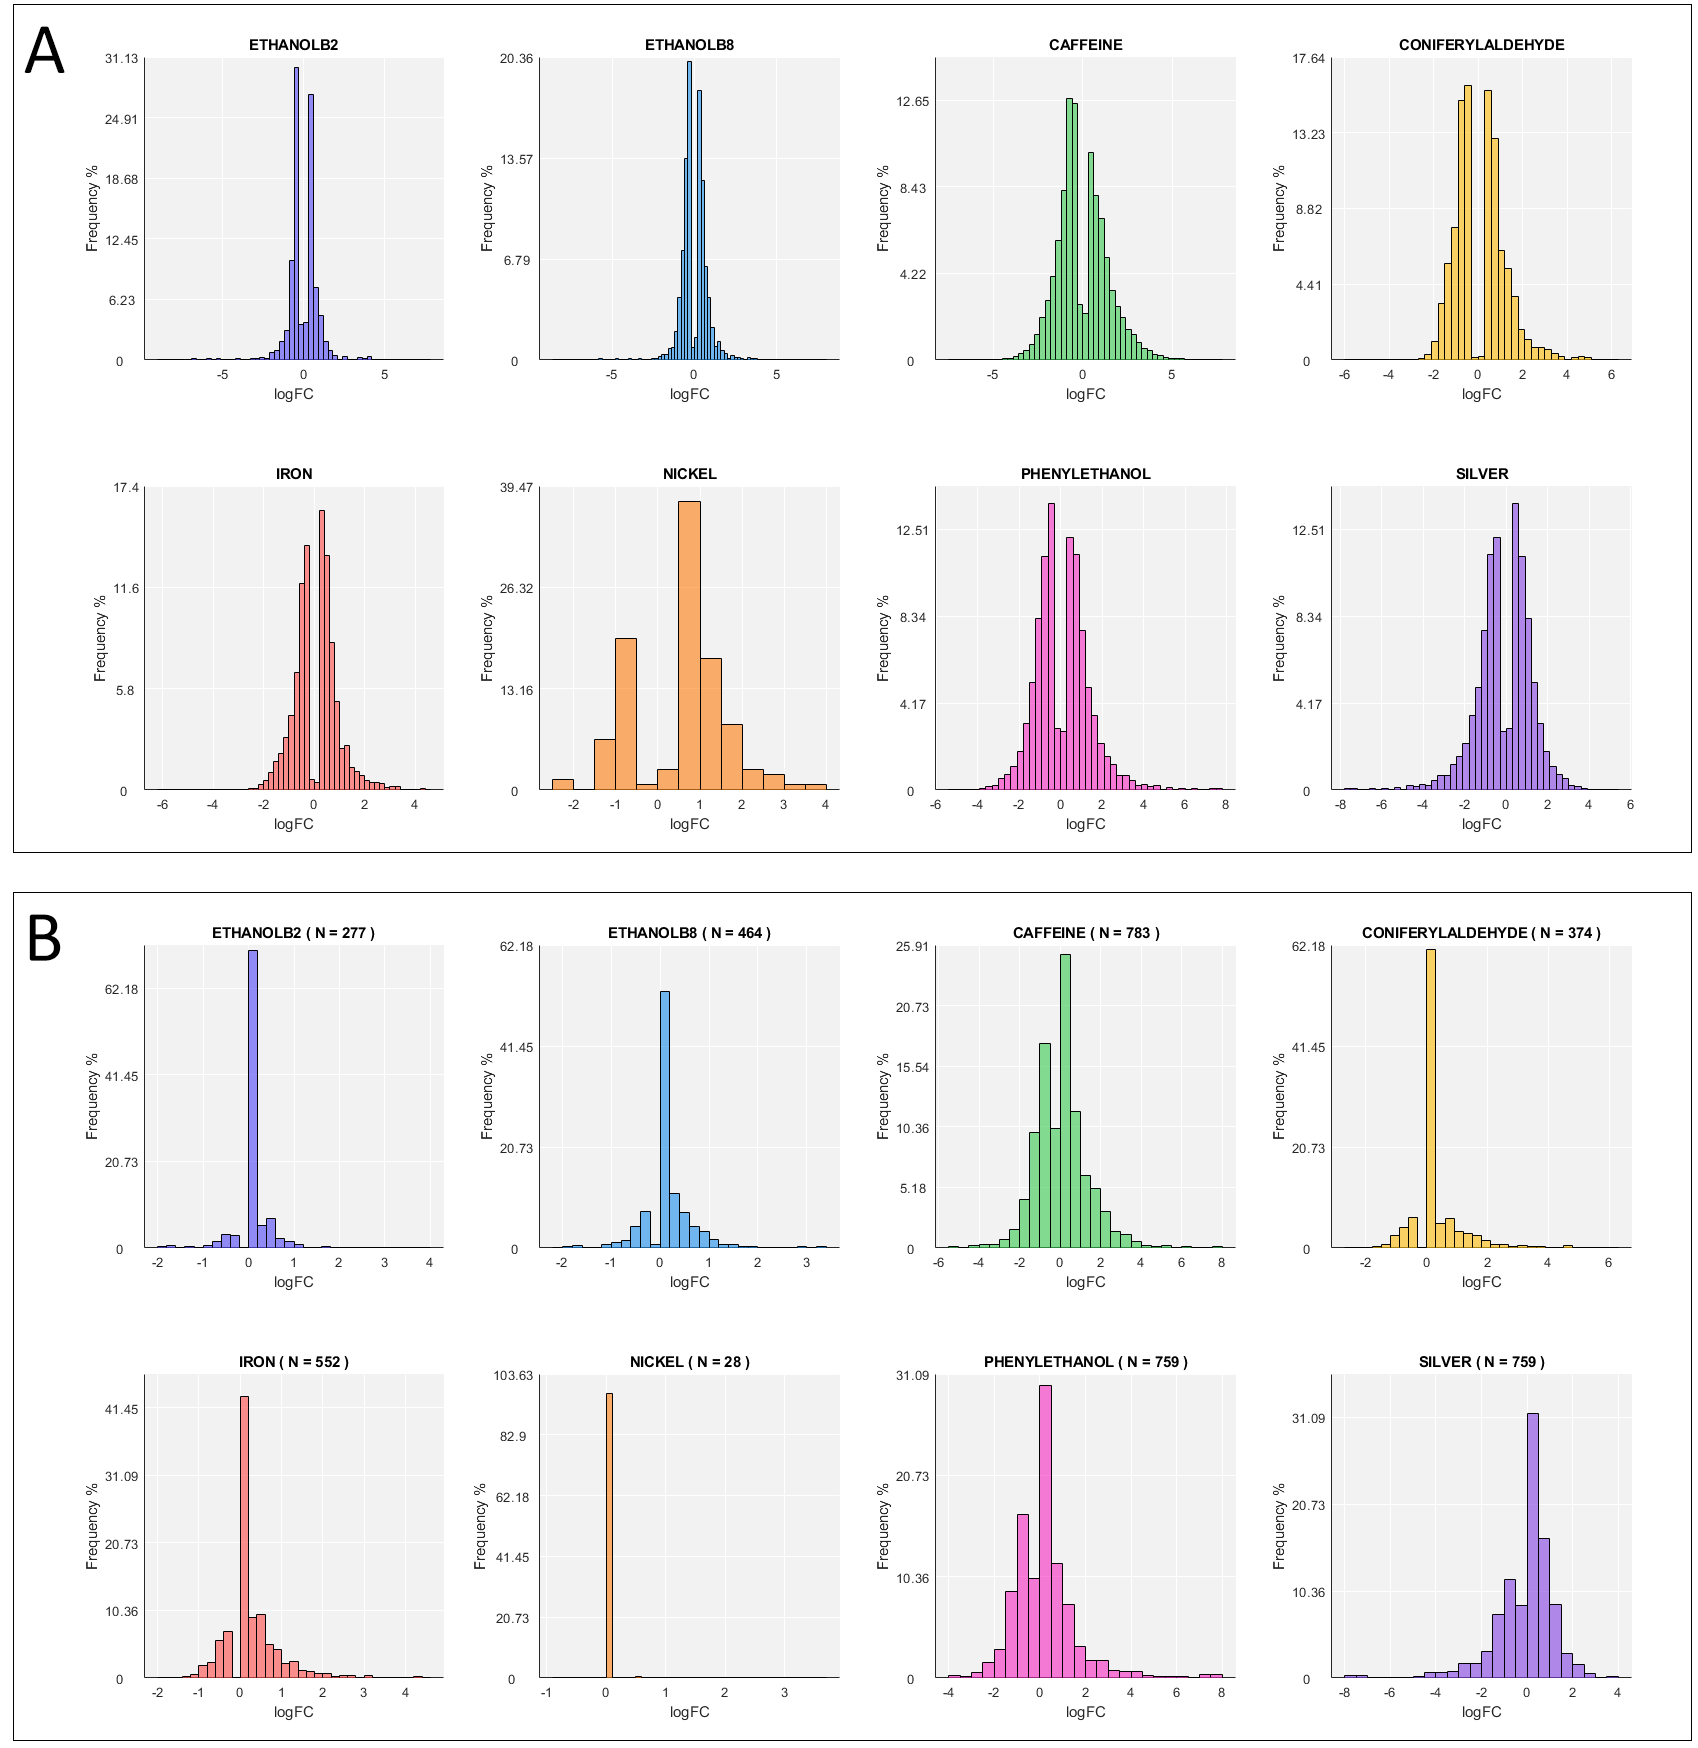
\includegraphics[width=1\columnwidth]{figures/expr_frequencies.png}
\caption[Frequencies of the differentially expressed genes]{Frequencies of the differentially expressed genes in A. Frequencies of the integrated genes in B.}
\end{center}
\label{fig:expr_frequencies}
\end{figure}

In order to validate the expression data integration method, fluxes for each enzyme (i.e. protein flux from protein pool to reaction for each protein) is predicted by flux balance analysis on all the strain models and on the wild-type model (wild-type here is referred as the metabolic model without expression data integrated). Flux ratios between wild-type and evolved models are calculated, and linear regression analysis is fitted after elimination of the outliers by the generalized extreme studentized deviate test to compare the flux-changes with the protein fold-changes from the expression data. Results confirm a good correlation between simulations and protein fold-change values (Figure \ref{fig:expr_linear_regressions}).

\begin{figure}[H]
\begin{center}
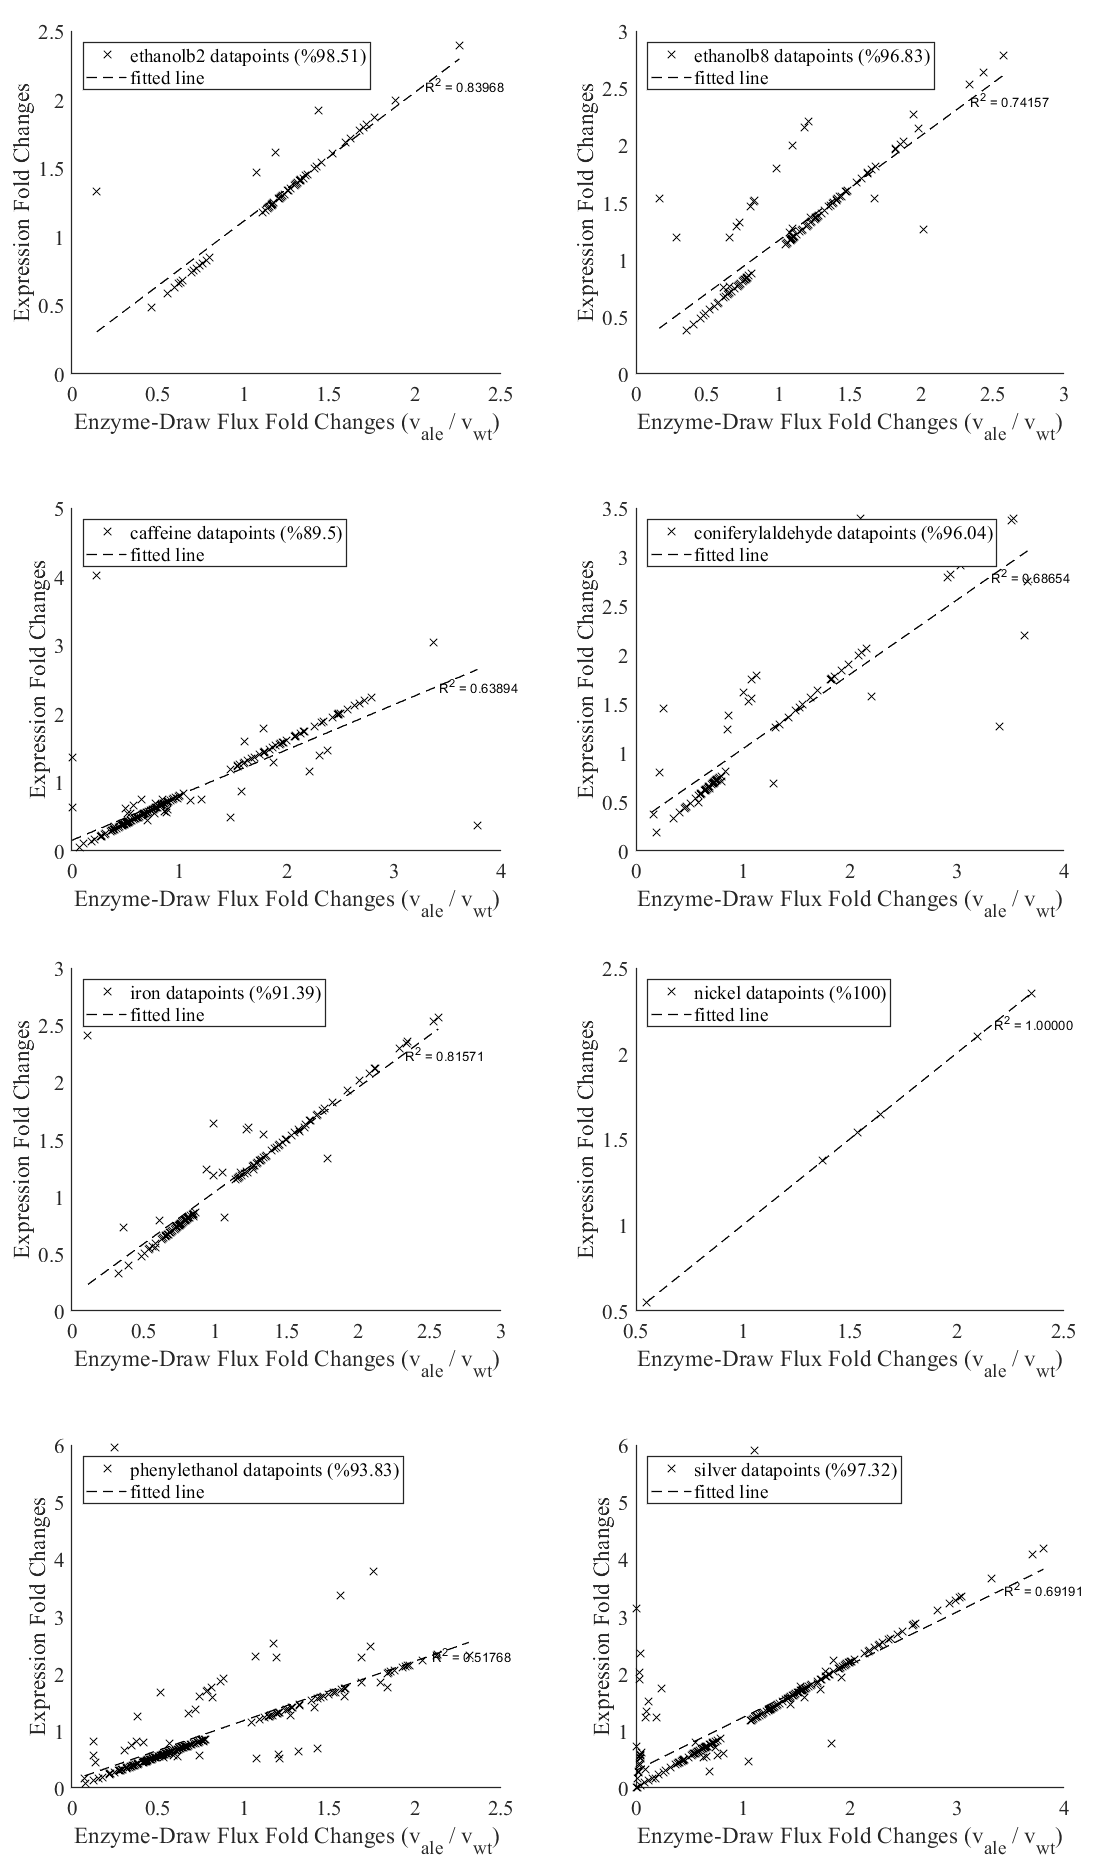
\includegraphics[width=1\columnwidth]{figures/expr_linear_regressions.png}
\caption[Linear regression analyses of the fold-changes]{Linear regression analyses of the enzyme-draw flux fold-changes and differential expression fold-changes of corresponding proteins.}
\end{center}
\label{fig:expr_linear_regressions}
\end{figure}



\section{Flux Balance Analysis Simulations}

The metabolic model is first simulated without the integration of the expression data (this model will be referred as wild-type model). Since the model is already enzymatically constrained, the only additional constraint required is the total amout of enzymes available in the enzyme pool. All the lower bounds for reactions were set to 0, and the upper bounds were set to 1000, except for the enzyme pool reaction. By doing that, the model was set free to be able to allocate enzymes as the reactions require. Flux rates of several exchange reactions as a function of growth rate are plotted in Figure \ref{fig:wt_crabtree}.

A behavioral change is observed around the time when growth rate is approximately 0.3 h\textsuperscript{-1}. Since the model is simulated under fully areobic conditions (no constraints applied) and produces ethanol, this behavior can be explained by the Crabtree effect, where the yeast metabolism switches to perform both respiration and fermantation at the same time at a critical specific growth rate.

\begin{figure}[H]
\begin{center}
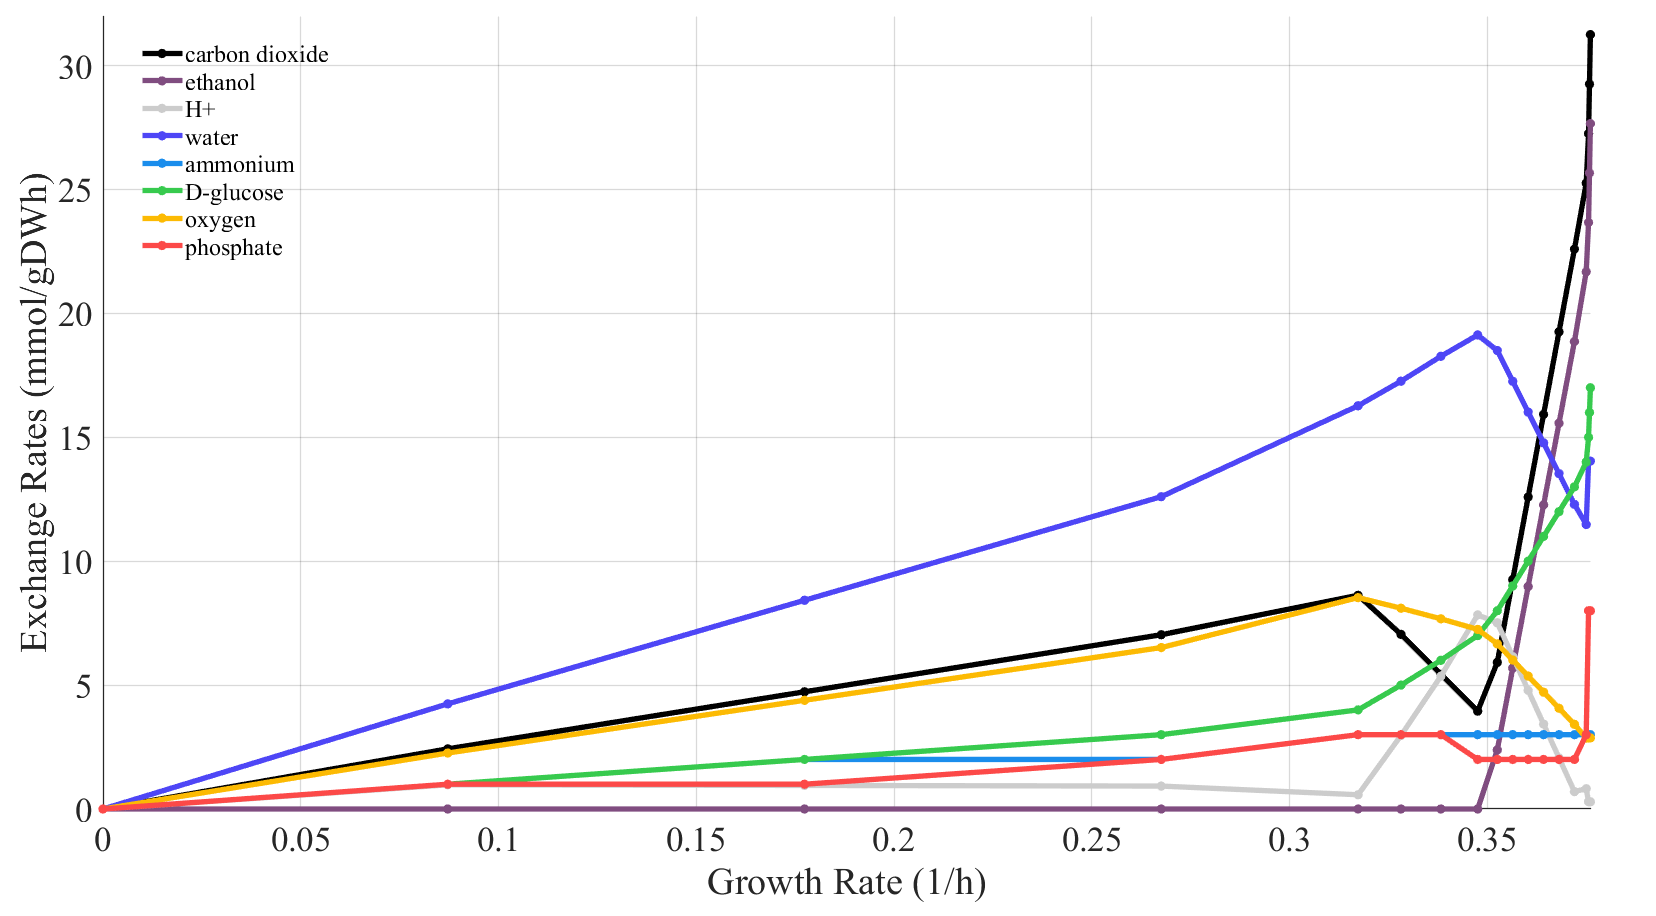
\includegraphics[width=1\columnwidth]{figures/wt_crabtree.png}
\caption[Metabolic model shows the overflow metabolism]{Metabolic model shows the overflow metabolism (crabtree effect) under fully aerobic conditions.}
\end{center}
\label{fig:wt_crabtree}
\end{figure}
\vspace{-1.0cm}

Robustness analysis is performed on the wild-type model for the growth rate with the varying levels of glucose uptake, oxygen uptake, acetate secretion and ethanol secretion rates (Figure \ref{fig:wt_robustness}). Unlike the traditional metabolic models, enzymatically constrained model showed non-linear graphs.

\begin{figure}[H]
\begin{center}
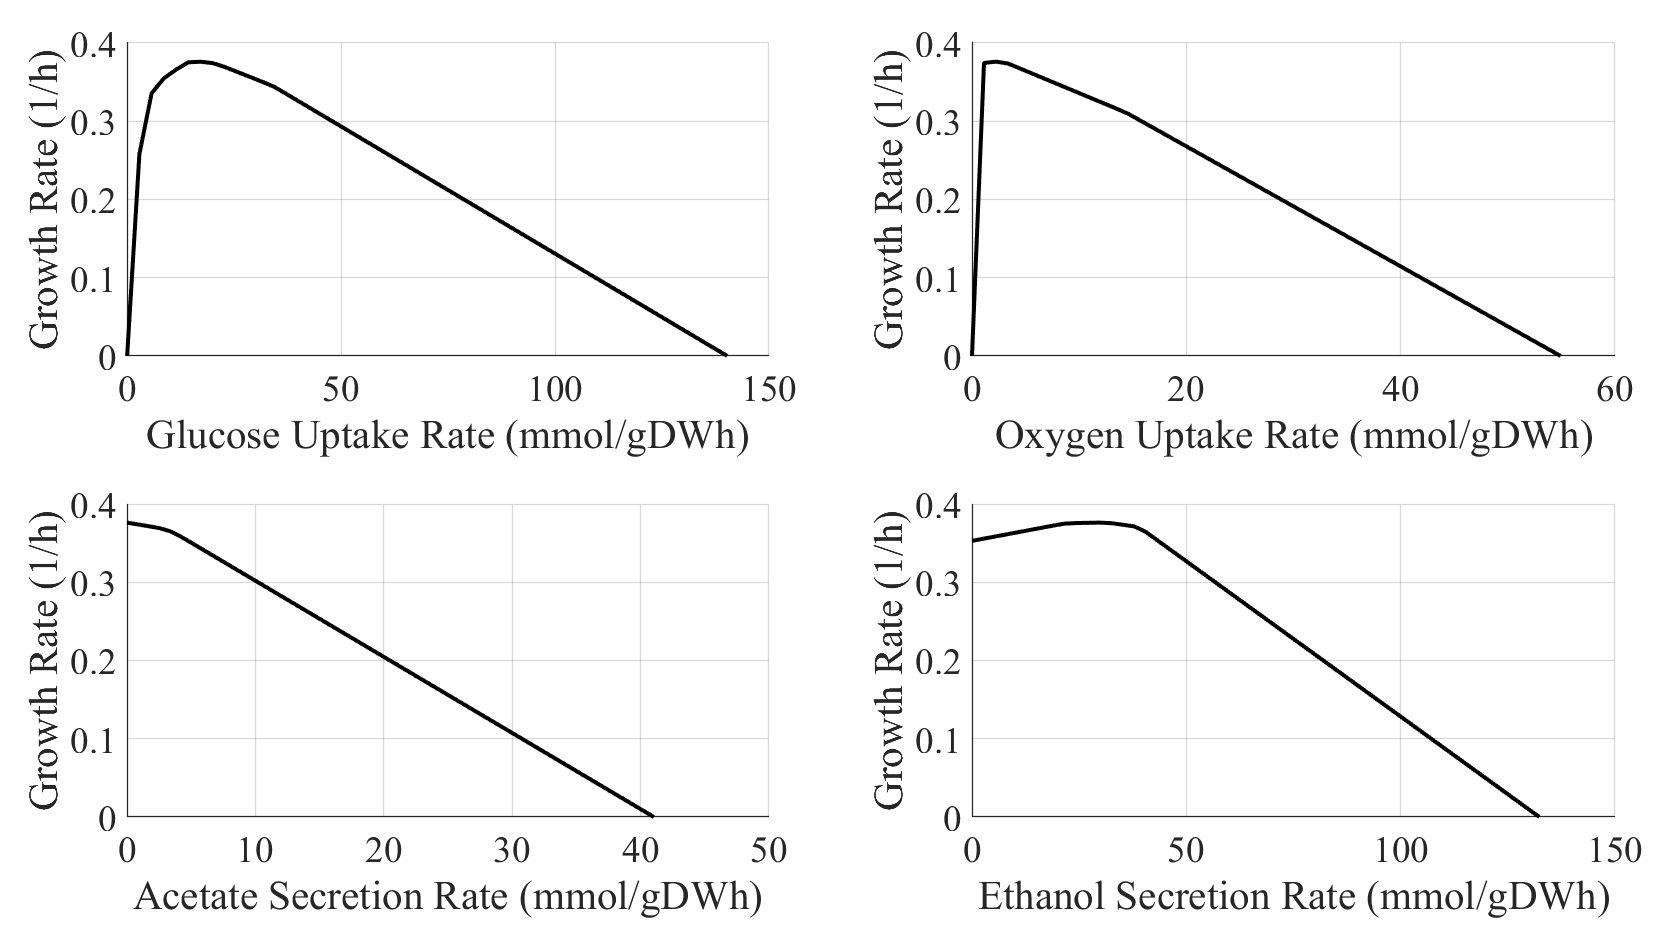
\includegraphics[width=1\columnwidth]{figures/wt_robustness.png}
\caption[Robustness analyses on the glucose uptake, oxygen uptake, acetate secretion and ethanol secretion rates]{Robustness analyses on the glucose uptake, oxygen uptake, acetate secretion and ethanol secretion rates.}
\end{center}
\label{fig:wt_robustness}
\end{figure}

\ifnotskip
For the anaerobic conditions, double robustness analysis of oxygen uptake and ethanol secretion rate is perfomed on the model to show the effect of oxygen availability on the system (Figure \ref{fig:v2_wt_robustness_ethanol}). The model predicted higher ethanol secretion under the lower oxygen availibility, as expected.

\begin{figure}[H]
\begin{center}
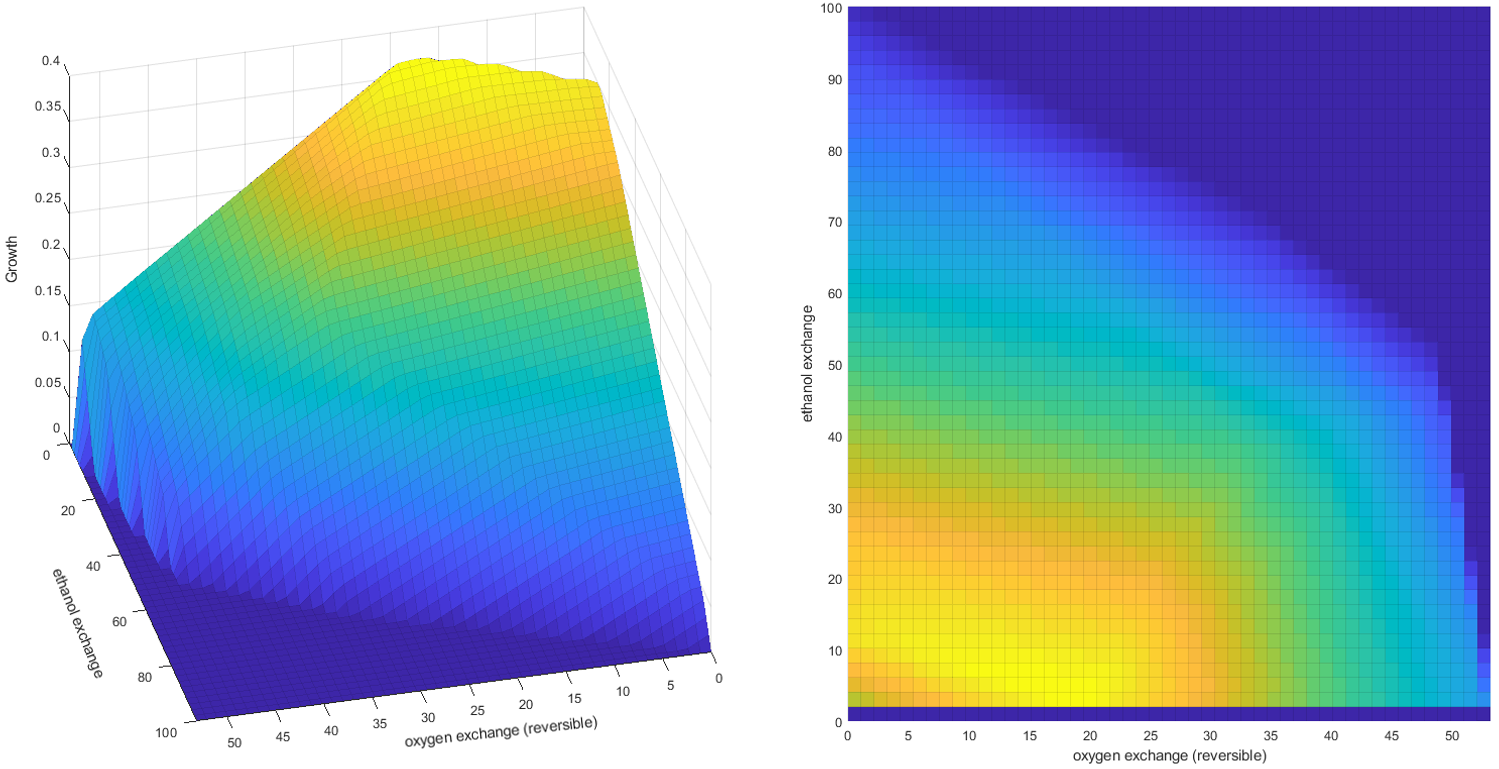
\includegraphics[width=0.8\columnwidth]{v2_wt_robustness_ethanol.png}
\caption[Double robustness analysis on oxygen uptake and ethanol secretion reactions]{Double robustness analysis on oxygen uptake and ethanol secretion reactions. (A) Phenotype phase-plane, (B) shadow prices of reactions.}
\end{center}
\label{fig:v2_wt_robustness_ethanol}
\end{figure}
\fi


After the validation of the wild-type model, all models for strains are simulated for the growth rates as a function of iteratively increasing glucose uptake rates (Figure \ref{fig:v2_fba_gur_vs_growth}). Models were able to grow up to the point where the protein accesibility becomes a limiting factor. It has been found that the evolved models except for the caffeine tolerant model show similar patterns on the points where proteins become limiting (break points in the lines). Ethanol tolerant model shows different pattern which it can consume more glucose to reach higher growth rates compared to others. Also it must be noted that while nacl and ethanol tolerant models can grow at higher rates than wild-type model, ethanol, iron, phenylethanol and nickel models can grow at lower rates.

\begin{figure}[H]
\begin{center}
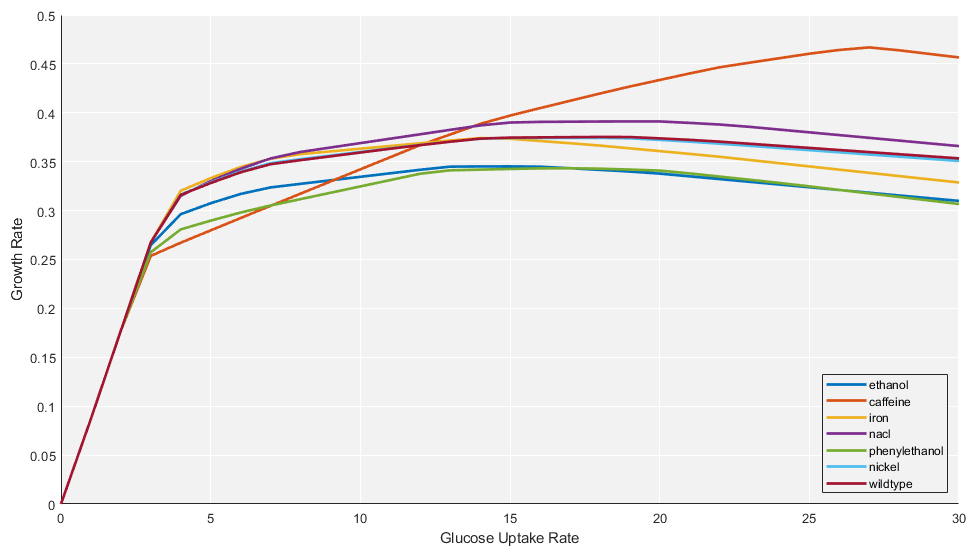
\includegraphics[width=1\columnwidth]{v2_fba_gur_vs_growth.png}
\caption[Growth rates as a function of iteratively increasing glucose uptake rates]{Growth rates as a function of iteratively increasing glucose uptake rates.}
\end{center}
\label{fig:v2_fba_gur_vs_growth}
\end{figure}
\vspace{-1.0cm}

In order to characterize differentiating points in the flux balance analysis solutions, cumulative flux vectors of each experiment are plotted (Figure \ref{fig:cumflux_free}). Standart deviations between strains for each reaction are calculated to find most diverging points.

\begin{figure}[H]
\begin{center}
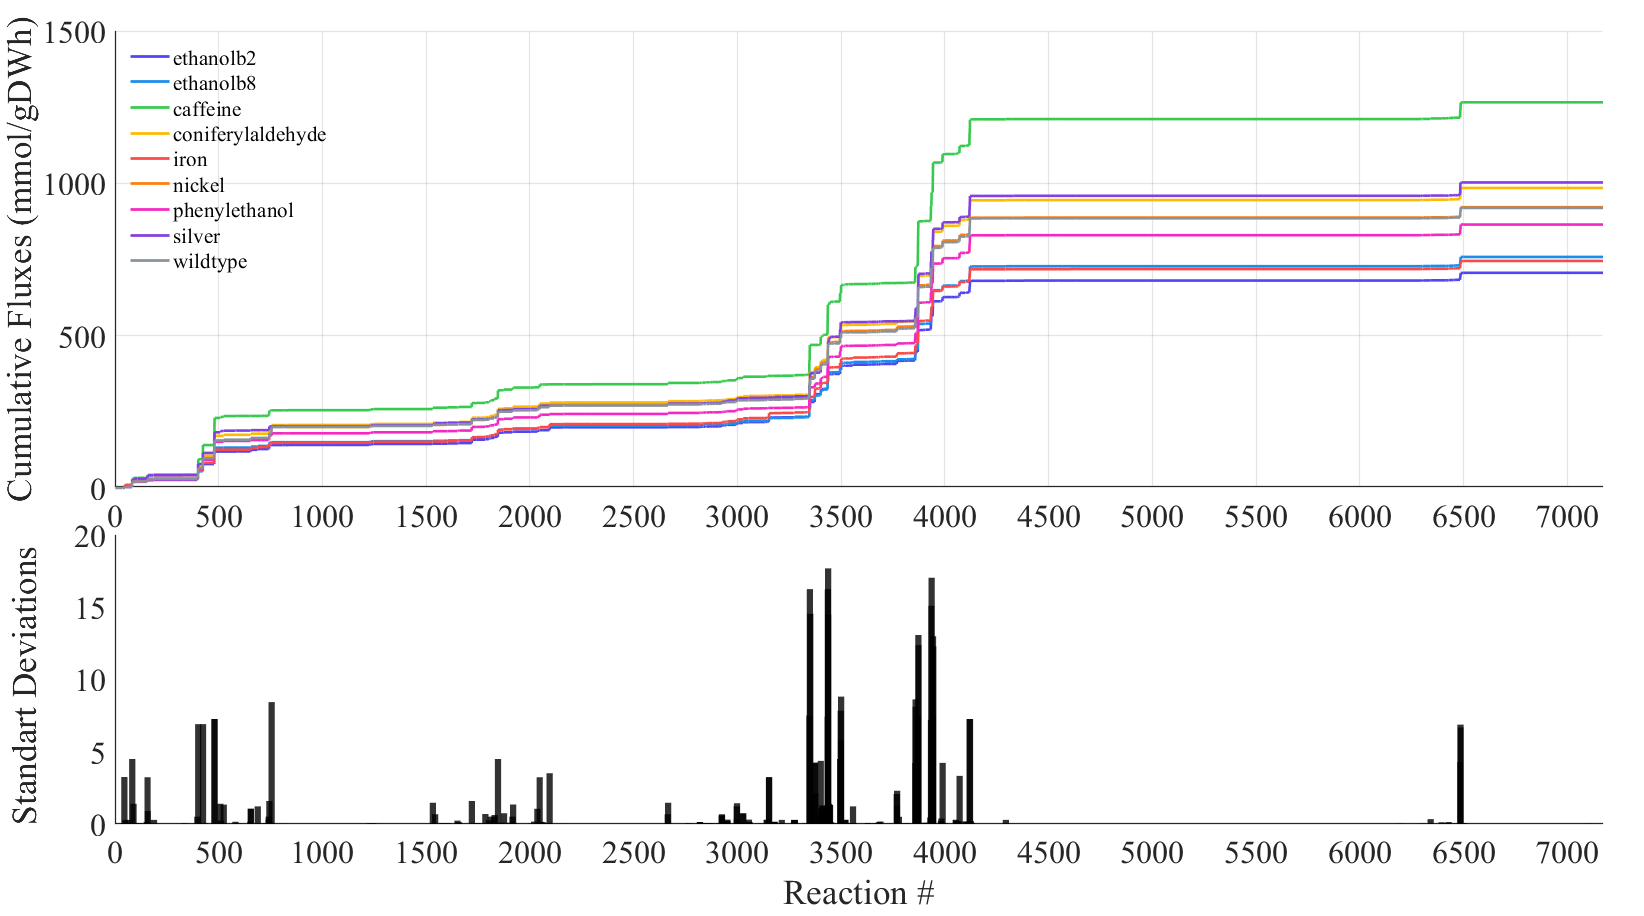
\includegraphics[width=1\columnwidth]{figures/cumflux_free.png}
\caption[Cumulative flux vectors of each simulation and standart deviations]{Cumulative flux vectors of each simulation and standart deviations.}
\end{center}
\label{fig:cumflux_free}
\end{figure}

Standart deviation values more then 10 are listed in Table \ref{table:cumulative_free_stds}

\begin{table}[H]
\caption[The most divergent reactions according to their standart deviations across all strains and their flux values in mmol/gDWh.]{The most divergent reactions according to their standart deviations across all strains and their flux values in mmol/gDWh.}
\begin{center}
  \setlength{\tabcolsep}{4pt}
  \resizebox{\textwidth}{!}{
  \begin{tabular}{cclcccccccccc}
\textbf{Rank} & \textbf{Genes} & \textbf{Reaction Nams}                            & \textbf{ethanolb2} & \textbf{ethanolb8} & \textbf{caffeine} & \textbf{coniferylaldehyde} & \textbf{iron} & \textbf{nickel} & \textbf{phenylethanol} & \textbf{silver} & \textbf{wildtype} & \textbf{std} \\ \hline
1             & YJL052W        & glyceraldehyde-3-phosphate  dehydrogenase   (No2) & 24.13              & 0                  & 0                 & 36.82                      & 0             & 32.79           & 0                      & 37.4            & 32.87             & 17.69        \\
2             & YLR134W        & pyruvate decarboxylase (No3)                      & 0                  & 0                  & 44.31             & 0                          & 22.11         & 0               & 30.08                  & 0               & 0                 & 17.04        \\
3             & YGR192C        & glyceraldehyde-3-phosphate  dehydrogenase   (No1) & 0                  & 0                  & 48.77             & 0                          & 0             & 0               & 0                      & 0               & 0                 & 16.26        \\
4             & YGR254W        & enolase (No2)                                     & 23.84              & 0                  & 48.77             & 36.5                       & 25.04         & 32.49           & 32.46                  & 0               & 32.56             & 16.25        \\
5             & YLR044C        & pyruvate decarboxylase (No2)                      & 20.94              & 25.19              & 0                 & 33.69                      & 0             & 29.42           & 0                      & 35.33           & 29.49             & 15.1         \\
6             & YMR323W        & enolase (No4)                                     & 0                  & 28.03              & 0                 & 0                          & 0             & 0               & 0                      & 37.13           & 0                 & 14.55        \\
7             & YJR009C        & glyceraldehyde-3-phosphate  dehydrogenase   (No3) & 0                  & 28.31              & 0                 & 0                          & 25.34         & 0               & 32.74                  & 0               & 0                 & 14.52        \\
8             & YOR283W        & phosphoglycerate mutase (No1)                     & 23.84              & 28.03              & 48.77             & 36.5                       & 25.04         & 32.49           & 32.46                  & 0               & 32.56             & 13.08        \\
9             & YAL038W        & pyruvate kinase (No1)                             & 23.6               & 27.79              & 48.45             & 36.24                      & 24.79         & 32.23           & 32.23                  & 0               & 32.31             & 12.99        \\
10            & YKL152C        & phosphoglycerate mutase (No2)                     & 0                  & 0                  & 0                 & 0                          & 0             & 0               & 0                      & 37.13           & 0                 & 12.38        \\
11            & YOR347C        & pyruvate kinase (No2)                             & 0                  & 0                  & 0                 & 0                          & 0             & 0               & 0                      & 36.9            & 0                 & 12.3
\end{tabular}}
\label{table:cumulative_free_stds}
\end{center}
\end{table}


Cumulative flux vectors of each experiment are plotted once more when the boundaries of the glucose uptake reaction is constrained to 10 gDWh\textsuperscript{-1} for each model (Figure \ref{fig:v2_fba_cumulative_gur10}). This has done to eliminate differences might be arising because of the free glucose uptake rates (as shown in below section, each model can uptake different maximum amount of glucose) and therefore affecting the downstream reaction fluxes.

\begin{figure}[H]
\begin{center}
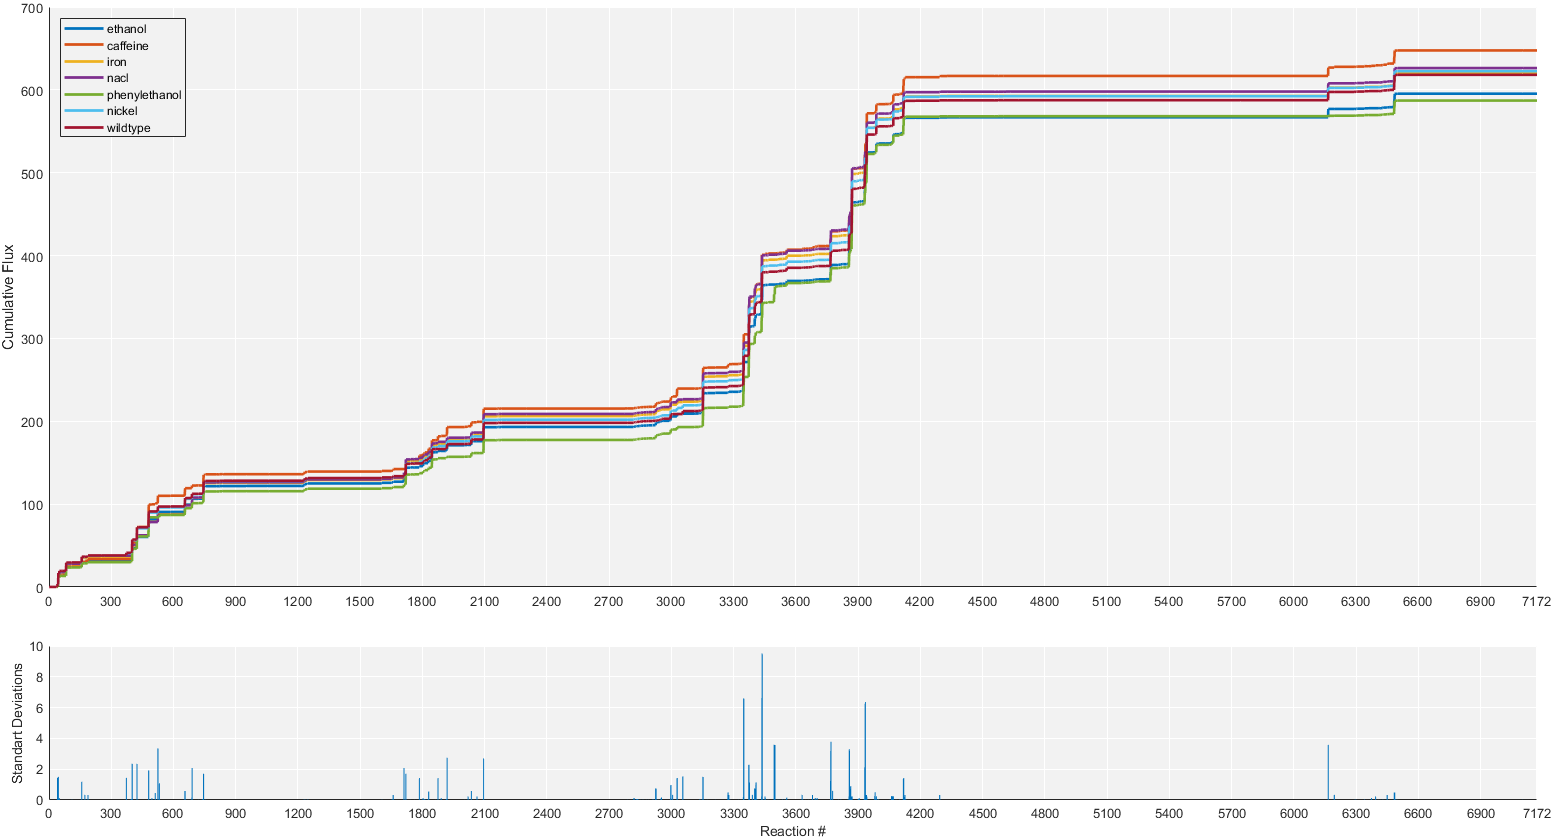
\includegraphics[width=1\columnwidth]{v2_fba_cumulative_gur10.png}
\caption[Cumulative flux vectors of each experiment when glucose uptake rate is constrained]{Cumulative flux vectors of each simulation and standart deviations. Glucose uptake rate is constrainted to  10 gDWh\textsuperscript{-1} for all models. }
\end{center}
\label{fig:v2_fba_cumulative_gur10}
\end{figure}


\section{Flux Variability Analysis}
Flux ranges of each enzyme on models are analyzed by the linear problem in the Flux Variability Analysis method where the objective functions to minimize and maximize all reactions iteratively with growth as the objective function kept at 90\%. Minimum and maximum available fluxes are collected in the iterative process for each reaction, and results are plotted in Figure \ref{fig:v2_fva}). Standart deviations on flux ranges for each reaction are also plotted to find most divergent targets. The most divergent proteins (top 20) across all experiments are collected in Table \ref{table:fva_results}.

\begin{figure}[H]
\begin{center}
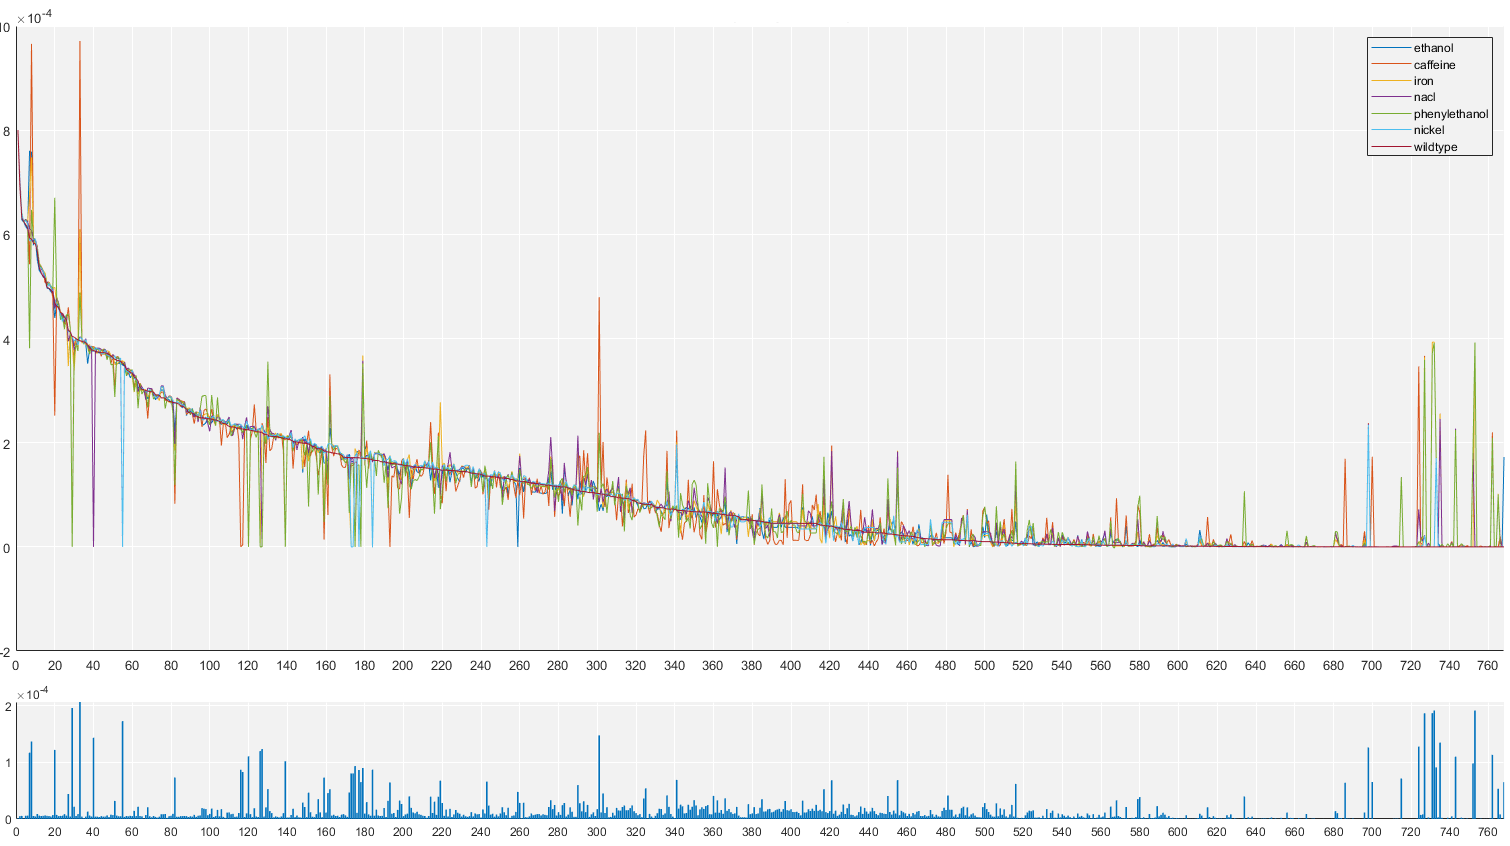
\includegraphics[width=1\columnwidth]{v2_fva.png}
\caption[Flux variability analysis]{Flux variability analysis results sorted by the wild-type flux ranges.}
\end{center}
\label{fig:v2_fva}
\end{figure}
\begin{table}[H]
\footnotesize
\caption[The most (std $>$ 55 nmol/gDWh) divergent proteins across all experiments and their flux variabilities as ranges (max - min flux) in nmol/gDWh]{The most (std $>$ 55 nmol/gDWh) divergent proteins across all experiments and their flux variabilities as ranges (max - min flux) in nmol/gDWh.}
\vspace{0.3cm}
\begin{center}
  \setlength{\tabcolsep}{4pt}
  \resizebox{\textwidth}{!}{
  \begin{tabular}{|c|c|c|c|c|c|c|c|c|c|c|}
    \hline
\textbf{Enzyme} & \textbf{b2-ethanol} & \textbf{b8-ethanol} & \textbf{caffeine} & \textbf{\begin{tabular}[c]{@{}l@{}}coniferyl \\ aldehyde\end{tabular}} & \textbf{iron} & \textbf{nickel} & \textbf{\begin{tabular}[c]{@{}l@{}}phenyl \\ ethanol\end{tabular}} & \textbf{silver} & \textbf{reference} & \textbf{std} \\ \hline

%
GRX1            & 580.52             & 798.71             & 796.91            & 799.92                     & 799.02        & 580.52          & 799.86                 & 0               & 580.52            & 261.34       \\ \hline
GRX2            & 580.52             & 580.52             & 622.01            & 624.36                     & 623.65        & 580.52          & 622.86                 & 0.08            & 580.52            & 201.73       \\ \hline
TDH3            & 561.29             & 609.88             & 968.54            & 403.74                     & 610.11        & 404.14          & 488.51                 & 296.71          & 403.66            & 196.83       \\ \hline
TDH2            & 702.15             & 760.74             & 965.83            & 607.13                     & 742.34        & 584.58          & 649.07                 & 305.09          & 586.70            & 177.49       \\ \hline
HYR1            & 530.62             & 530.44             & 529.25            & 531.24                     & 530.65        & 531.78          & 529.97                 & 0               & 531.14            & 176.88       \\ \hline
GPX1            & 507.66             & 507.49             & 506.35            & 508.26                     & 507.69        & 508.74          & 507.04                 & 0               & 508.16            & 169.23       \\ \hline
TDH1            & 704.05             & 762.80             & 542.42            & 606.64                     & 672.41        & 586.16          & 381.54                 & 315.49          & 588.29            & 145.14       \\ \hline
OLI1            & 498.12             & 447.32             & 256.85            & 462.14                     & 503.37        & 480.46          & 668.93                 & 177.89          & 471.85            & 143.72       \\ \hline
TRX2            & 83.56              & 76.81              & 477.59            & 85.43                      & 91.79         & 101.72          & 218.84                 & 43.53           & 102.17            & 134.54       \\ \hline
SOL4            & 239.80             & 324.14             & 363.99            & 365.53                     & 377.35        & 156.46          & 351.92                 & 18.15           & 164.11            & 126.02       \\ \hline
ERG10           & 237.06             & 236.98             & 0.01              & 0.02                       & 0.02          & 214.75          & 0.01                   & 238.31          & 237.27            & 122.94       \\ \hline
CYC7            & 3.07               & 6.00               & 345.15            & 72.74                      & 10.38         & 1.24            & 15.25                  & 0.07            & 0.55              & 112.84       \\ \hline
AYR1            & 274.31             & 301.45             & 301.68            & 63.66                      & 301.41        & 301.16          & 26.45                  & 302.96          & 301.69            & 112.20       \\ \hline
PGA3            & 280.31             & 280.22             & 279.59            & 280.28                     & 280.33        & 280.16          & 0                      & 281.75          & 280.59            & 93.47        \\ \hline
SNO3            & 0                  & 0                  & 0                 & 0                          & 0             & 0               & 0                      & 261.32          & 0                 & 87.11        \\ \hline
DAS2            & 259.51             & 224.29             & 96.71             & 211.09                     & 191.35        & 276.99          & 126.60                 & 363.82          & 279.13            & 81.82        \\ \hline
HXK1            & 82.23              & 146.33             & 188.50            & 189.24                     & 193.89        & 33.59           & 186.56                 & 0.01            & 34.44             & 79.54        \\ \hline
SNO2            & 0                  & 0                  & 0                 & 0                          & 0             & 0               & 0                      & 237.53          & 0                 & 79.18        \\ \hline
URA6            & 153.11             & 148.21             & 113.37            & 133.15                     & 123.92        & 175.63          & 76.48                  & 349.32          & 179.93            & 77.32        \\ \hline
YDC1            & 265.82             & 137.27             & 265.96            & 265.85                     & 265.50        & 265.13          & 265.98                 & 261.85          & 58.55             & 76.34        \\ \hline
YOR283W         & 385.25             & 284.27             & 374.59            & 386.44                     & 383.88        & 167.70          & 354.85                 & 391.22          & 387.67            & 74.91        \\ \hline
SOL3            & 173.27             & 160.34             & 102.97            & 127.45                     & 116.01        & 161.25          & 62.84                  & 307.74          & 165.03            & 68.26        \\ \hline
CDC8            & 180.45             & 172.85             & 222.25            & 182.36                     & 168.37        & 198.14          & 78.50                  & 336.56          & 201.04            & 67.03        \\ \hline
ALG13           & 222.59             & 233.87             & 342.51            & 266.53                     & 268.81        & 198.78          & 292.49                 & 113.05          & 199.23            & 65.73        \\ \hline
GPX2            & 537.40             & 537.23             & 536.02            & 341.26                     & 537.43        & 538.58          & 488.86                 & 540.21          & 537.93            & 65.52        \\ \hline
PDC5            & 157.75             & 161.29             & 17.12             & 185.99                     & 76.60         & 181.67          & 48.37                  & 169.86          & 183.92            & 65.47        \\ \hline
GLK1            & 27.76              & 50.03              & 133.67            & 135.09                     & 92.54         & 33.06           & 193.48                 & 0               & 34.35             & 64.44        \\ \hline
GPP2            & 204.17             & 215.88             & 261.44            & 299.76                     & 230.49        & 212.94          & 355.61                 & 147.19          & 219.99            & 60.29        \\ \hline
ALD4            & 44.53              & 37.53              & 140.64            & 138.00                     & 78.24         & 40.30           & 174.06                 & 1.32            & 39.86             & 59.43        \\ \hline
PYK2            & 91.09              & 88.38              & 195.97            & 183.93                     & 169.19        & 55.15           & 108.01                 & 38.43           & 56.16             & 59.39        \\ \hline
ALG14           & 179.10             & 169.99             & 77.84             & 142.43                     & 140.31        & 198.78          & 120.83                 & 273.04          & 199.23            & 55.73        \\ \hline
MHT1            & 107.29             & 91.30              & 170.34            & 216.78                     & 183.08        & 108.03          & 41.78                  & 171.04          & 108.32            & 55.14        \\ \hline

\end{tabular}}
\label{table:fva_results}
\end{center}
\end{table}



\section{Enzyme Essentiality}
To calculate the essentiality of the proteins, \emph{in-silico} single reaction deletion analysis is applied to the protein draw reactions on all models. The impacts of the enzyme deletions on growth (as the objective function) of the most essential (top 10) proteins are plotted in Figure \ref{fig:v2_proteinknockout}.

\begin{figure}[H]
\begin{center}
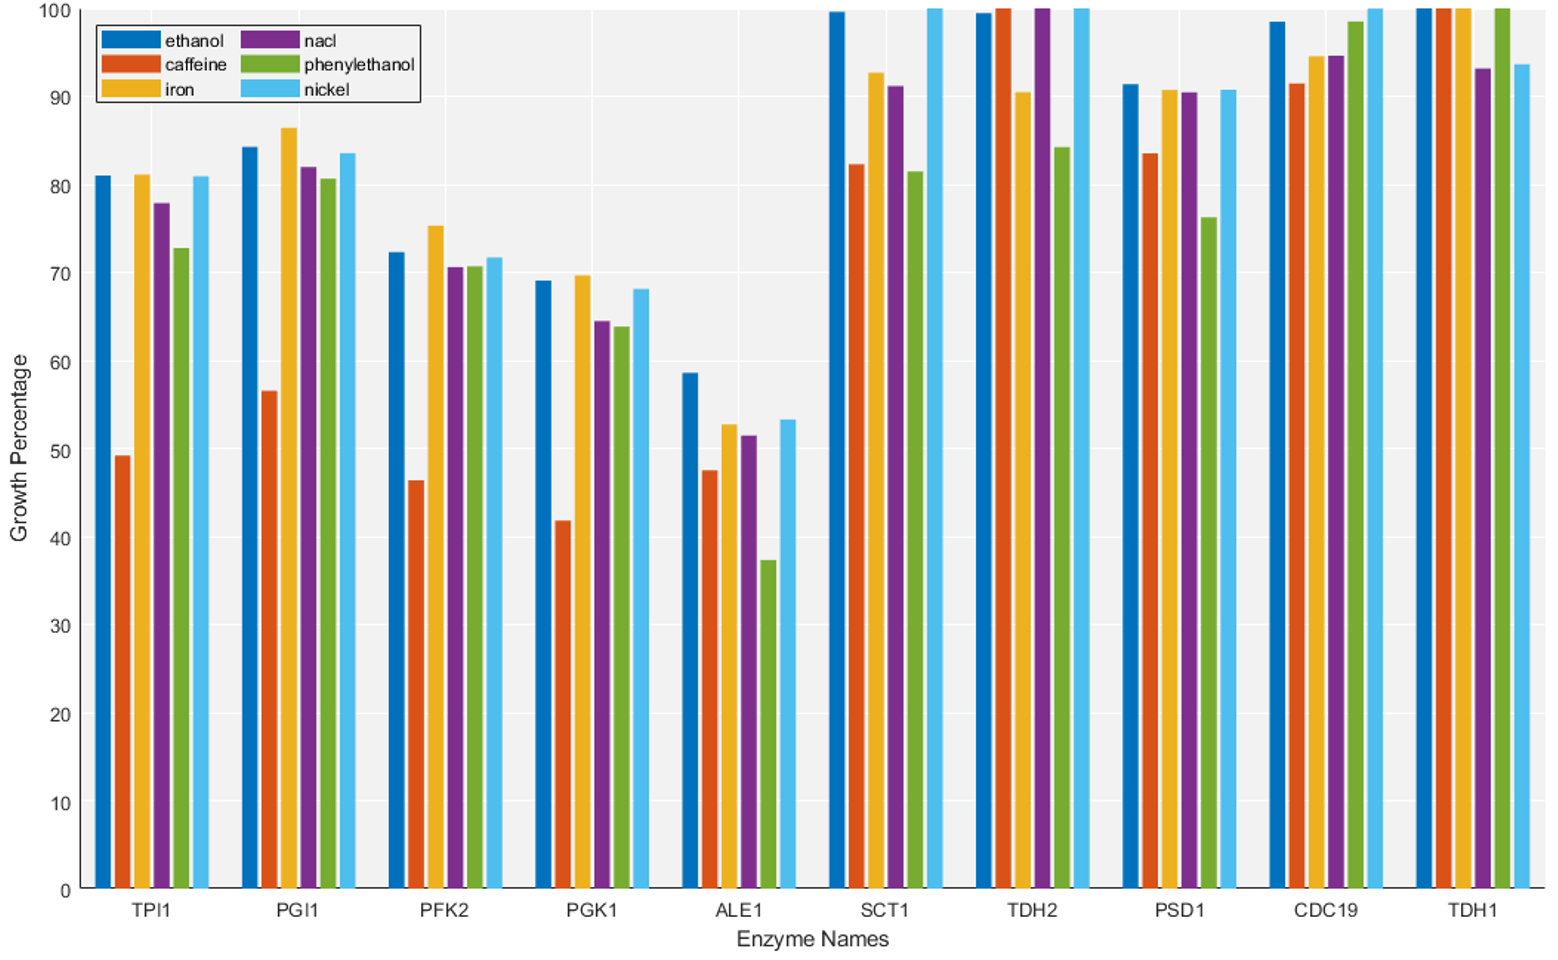
\includegraphics[width=1\columnwidth]{v2_proteinknockout.png}
\end{center}
\caption[Important protein targets and their knock-out effects on growth rate]{Important protein targets and their knock-out effects on growth rate.}
\label{fig:v2_proteinknockout}
\end{figure}


\section{Minimization of Metabolic Adjustment}

MOMA results are investigated for the metabolic reactions and the protein draw reactions seperately. Flux distances for each reaction of evolved models to the wild type models are calculated and plotted (Figure \ref{fig:v2_moma_cumdist}). The top 5 ranked reactions for the maximum cumulative distance from the wild type fluxes found as palmitoyl-CoA hydrolase, long chain fatty acid CoA ligase, carbon dioxide exchange, glyceraldehyde-3-phosphate dehydrogenase, methylglyoxal synthase reactions. On the other hand, the enzymes TDH1 (glyceraldehyde-3-phosphate dehydrogenase isozyme 1), RIB7 (Diamino-hydroxy-phoshoribosyl-amino-pyrimidine deaminase), GPT2 (glycerol-3-phosphate/dihydroxyacetone phosphate sn-1 acyltransferase), SCT1(glycerol 3-phosphate/dihydroxyacetone phosphate sn-1 acyltransferase) and SEC53 (phosphomannomutase) were the top 5 ranked enzymes.

\begin{figure}[H]
\begin{center}
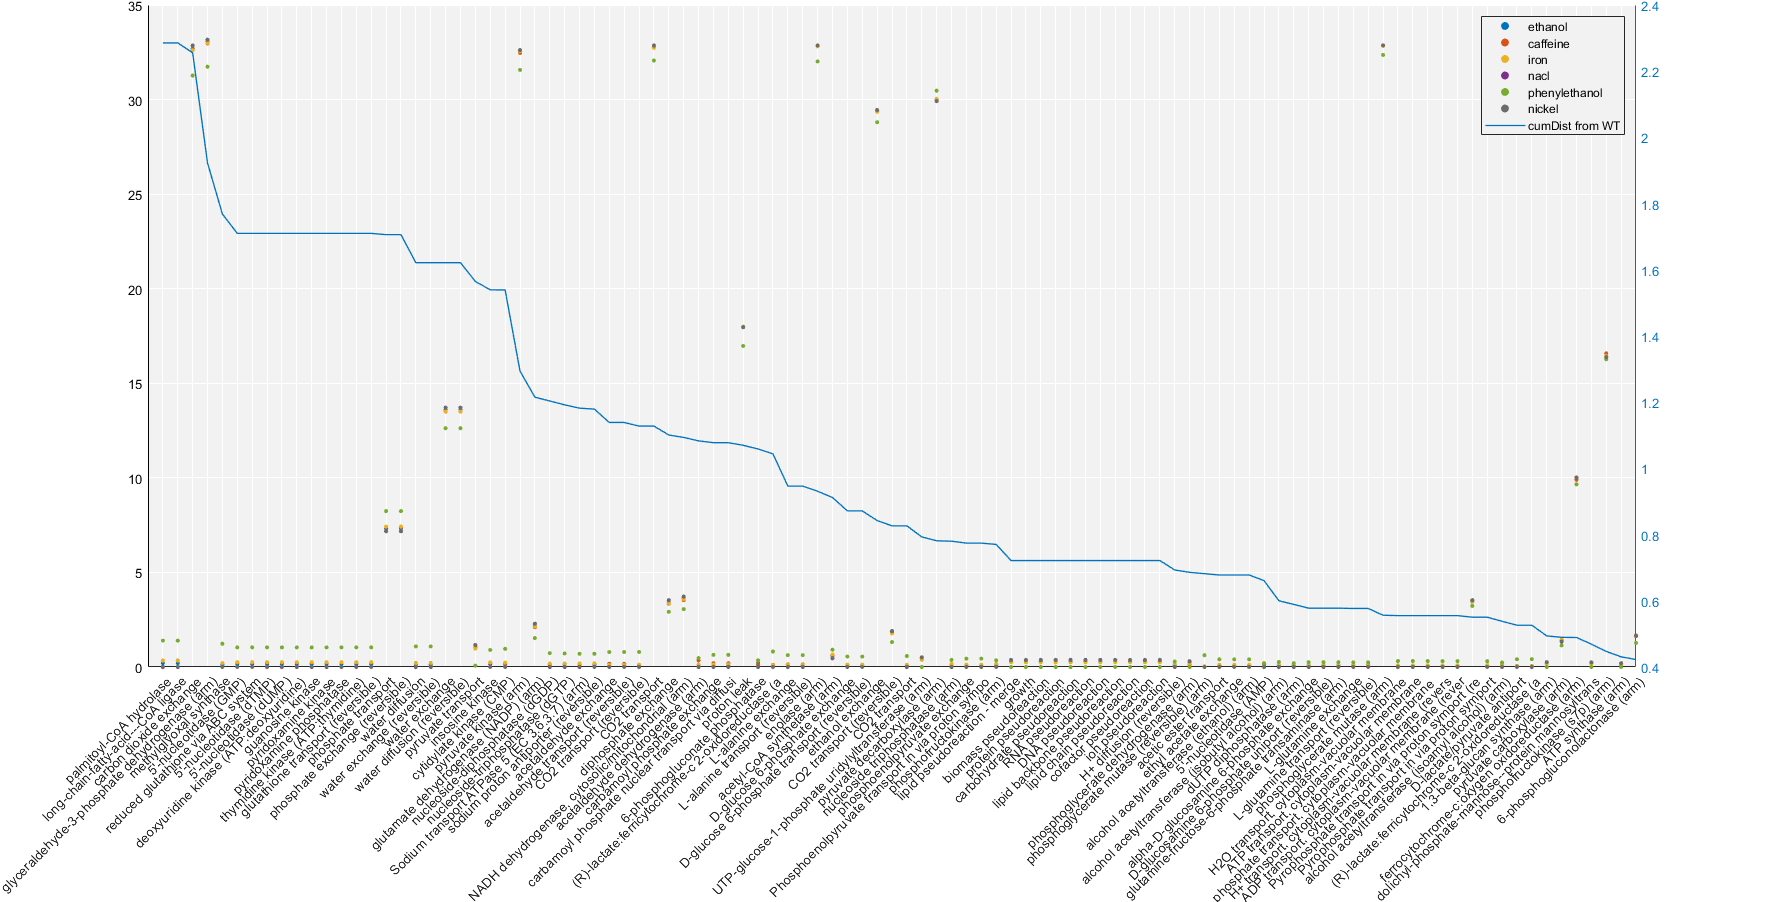
\includegraphics[width=1\columnwidth]{v2_moma_cumdist.png}
\noindent\rule{14cm}{0.4pt}
\vskip\baselineskip
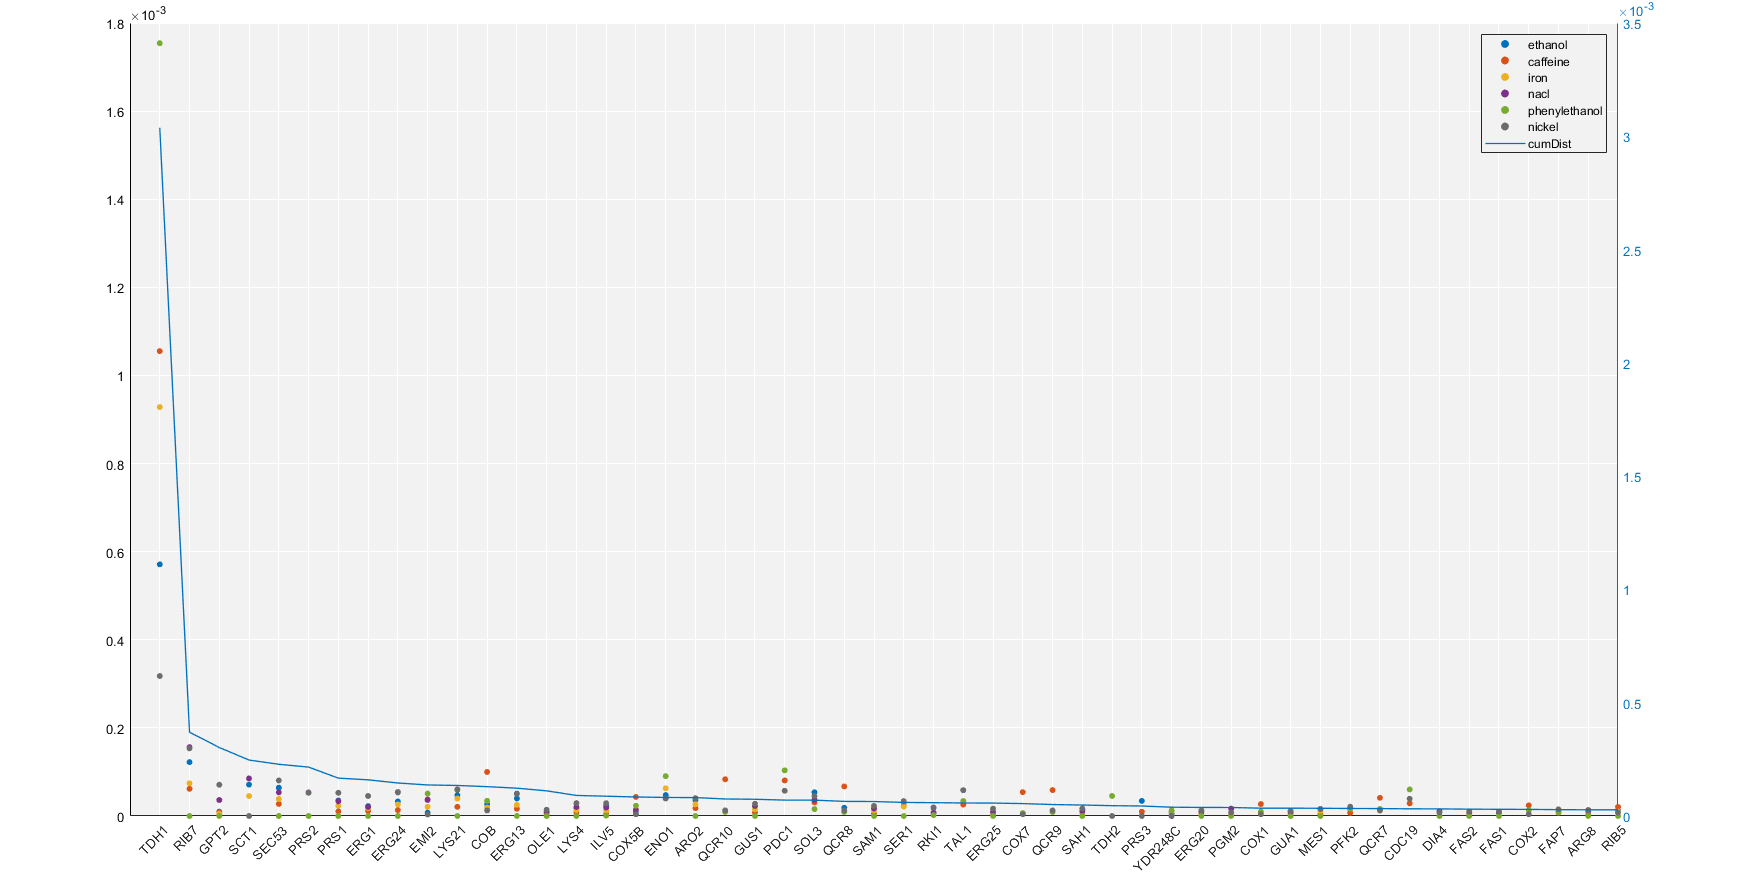
\includegraphics[width=1\columnwidth]{v2_moma_cumdist_prot.png}
\end{center}
\caption[Reactions and proteins that has MOMA fluxes the most distant from the wild-type fluxes]{Reactions (top) and proteins (bottom) that have MOMA flux values the most distant from the wild-type flux values.}
\label{fig:v2_moma_cumdist}
\end{figure}


\section{Sampling Results}
I was not able to sample solution spaces correctly, yet.
